%%%%%%%%%%%%%%%%%%%%%%%%%%%%%% -*- Mode: Latex -*- %%%%%%%%%%%%%%%%%%%%%%%%%%%%
%% main.tex<fourier_decomp> -- 
%% Last Modified On: Thu Apr 13 16:15:17 2023 (+0200)
%%%%%%%%%%%%%%%%%%%%%%%%%%%%%%%%%%%%%%%%%%%%%%%%%%%%%%%%%%%%%%%%%%%%%%%%%%%%%%%

\documentclass[final]{zamarep}

% Useful LaTeX packages
\usepackage{mathtools}
\usepackage{mathcalbd} % for \pol macro

\usepackage[colorlinks]{hyperref} % should be loaded last
\usepackage{cleveref}  % should be loaded last last

\title{Verifiable FHE Prototype}
\subtitle{Documentation}

\author[MW]{Michael Walter}

% \date{April 13, 2023}

%\titlegraphic[credit={Erik Karits}]{%
%  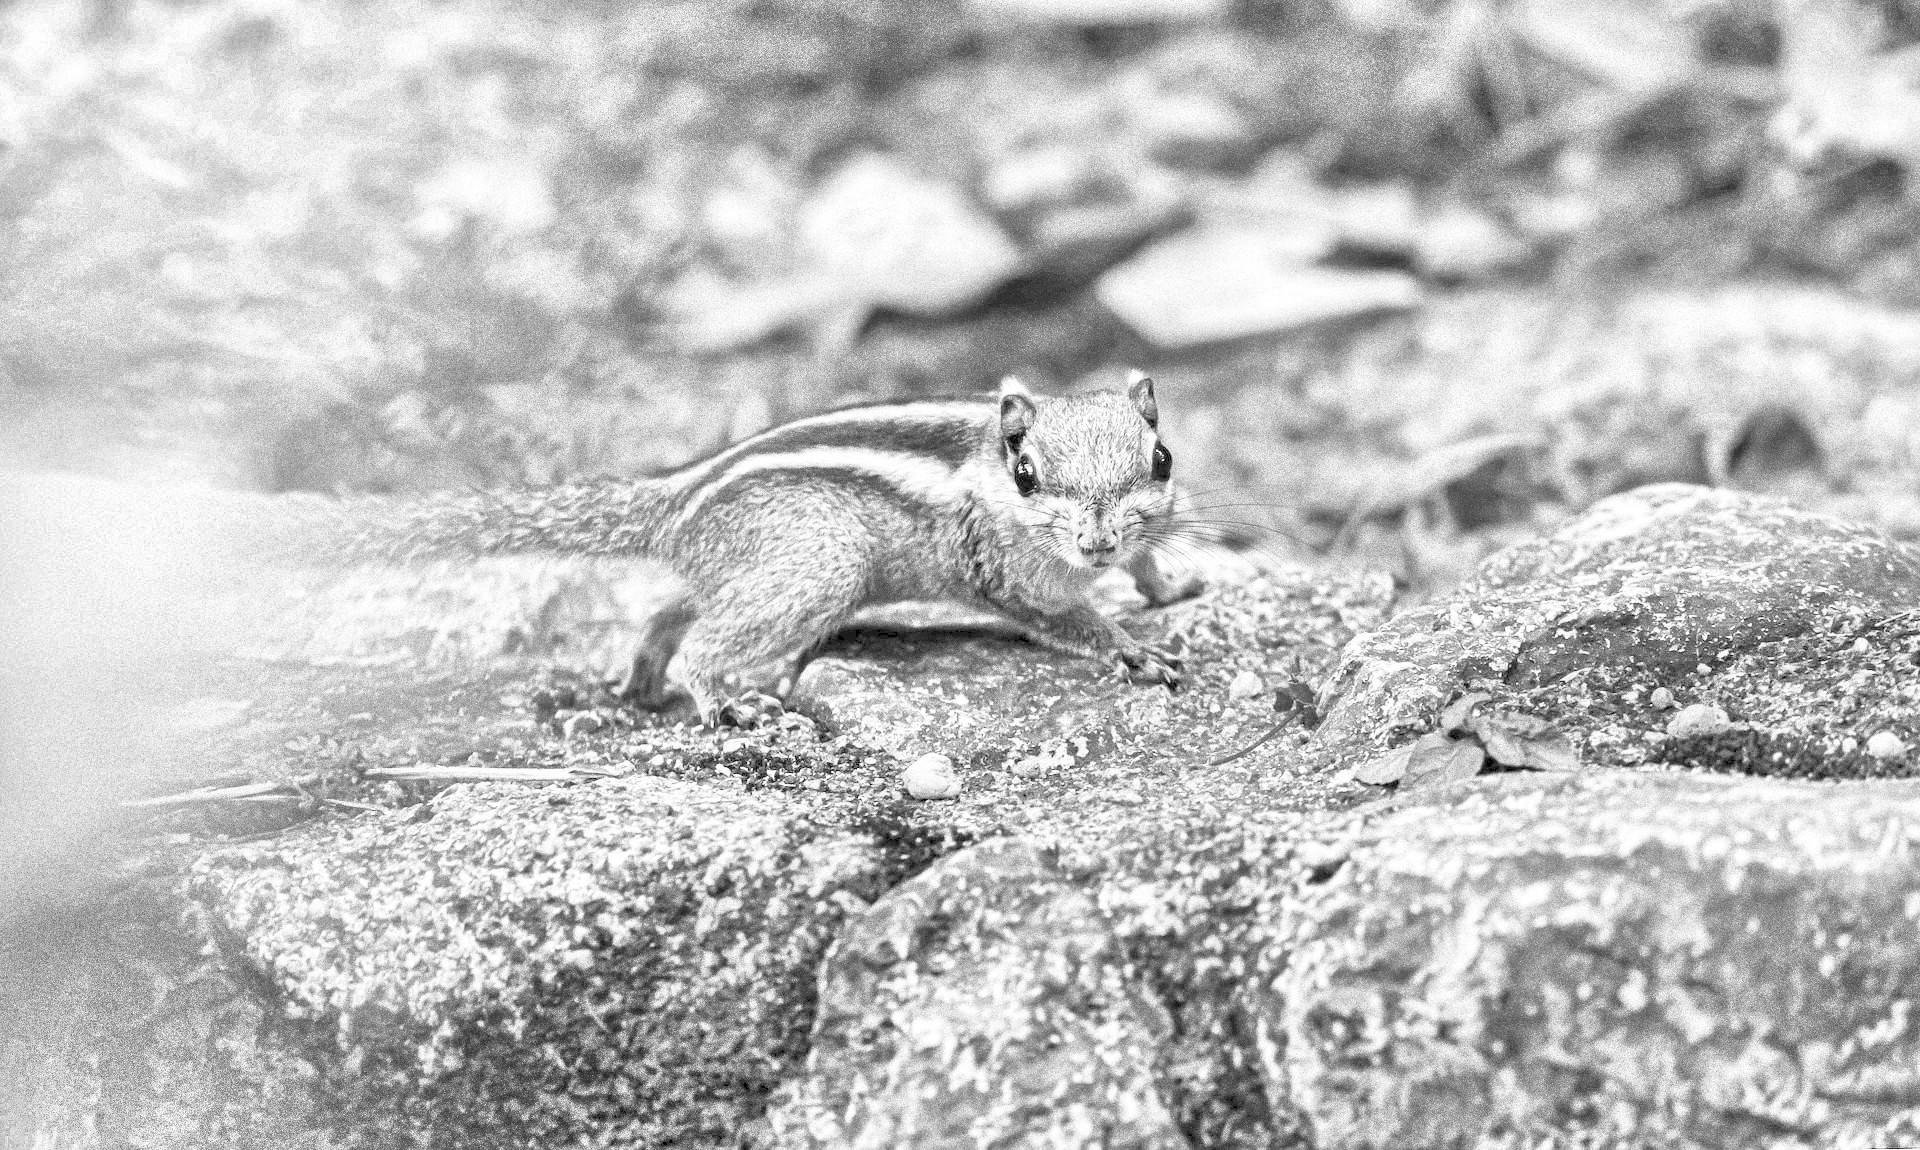
\includegraphics{erik-karits-Ivy_nqt6gTc-unsplash}}


% --- Macros
% \newcommand{\ints}{\mathds{Z}}
% \newcommand{\reals}{\mathds{R}}
% \newcommand{\torus}{\mathds{T}}
% \newcommand*{\pol}{\mathcalbd}
% \newcommand*{\SQ}{\mathit{S\!Q}}

\newcommand{\field}{\mathbb{F}}
\newcommand{\sha}{\texttt{SHA256}~}
% \newcommand{\rs}[3]{\mathrm{RS()}}
\newcommand{\abs}[1]{\lvert #1 \rvert}
\newcommand{\Sel}[1]{S_{\mathrm{#1}}}
\newcommand{\psel}[1]{p_{\mathrm{#1}}}

\begin{document}

\maketitle

%%%%%%%%%%%%%%%%%%%%%%%%%%%%%%%%%%%%%%%%%%%%%%%%%%%%%%%%%%%%%%%%%%%%%%%%%%%%%%% 
\section{Introduction}\label{sec:introduction}
%%%%%%%%%%%%%%%%%%%%%%%%%%%%%%%%%%%%%%%%%%%%%%%%%%%%%%%%%%%%%%%%%%%%%%%%%%%%%%% 

This document describes the prototype of a verifiable FHE protocol implemented in Sage. The prototype is based on a general purpose SNARK, specifically on PLONK in combination with a FRI-based PCS. The goal of the protocol is to allow the FHE evaluator to prove the correct execution of an FHE circuit using the clients ciphertexts and evalutation keys.

The implementation can be viewed as consisting of three modules:
\begin{enumerate}
\item the FRI-based PCS, cf.\ Section \ref{sec:fri}
\item the PLONK arithemtization, cf.\ Section \ref{sec:plonk}
\item the circuit generation and translation to the PLONK format, cf.\ Section \ref{sec:circuit_gen}.
\end{enumerate}
The latter includes the circuit for the PBS, cf.\ Section \ref{sec:subcircuit}.

\section{Preliminaries}
\label{sec:prelims}
For an integer $k$ we denote by $[k]$ the set $\{0, 1, \dots, k-1\}$. Throughout we fix the field $\field$ to be $\field_p$ for some prime $p$. 

\subsection{Merkle Commitments}
\label{sec:merkle}

Merkle trees are standard cryptographic objects that allow to commit to a vector and subsequently open arbitrary points in the vector. In order to commit to a vector, a Merkle tree is computed from it by arranging the vector elements on the lowest layer. The layers are now computed recursively by merging two nodes in the previous layer into a new node by hashing their concatenation. The output of the hash is the corresponding label for the new node. This is done until the tree is complete. The root serves as the commitment to the vector and the vector may now be opened at some position by sending the siblings of the nodes along the path from the point to the root. The binding property of the Merle commitment relies on the collision resistance of the hash function.

\subsection{Fiat-Shamir Transform}
\label{sec:fs}

The Fiat-Shamir (FS) transform is a way to turn a public coin interactive protocol into a non-interactive protocol. The idea is to compute verifier challenges using a hash function from the messages exchanged so far. Not all public coin protocols are secure using the FS transform, but the protocols we will consider are, at least in the random oracle model \cite{DBLP:journals/iacr/BlockGKTTZ23}.

\section{FRI-based PCS}
\label{sec:fri}
FRI \cite{ICALP:BBHR18} is a protocol for proving that a polynomial has low degree. This protocol can then be turned into a polynomial commitment scheme, as we will outline in Section \ref{sec:pcs}.

On a high level, FRI works by using a Merkle commitment to commit to an Reed-Solomon (RS) encoding of a given polynomial, then ``folding'' the polynomial into a polynomial of half the size using a verifier challenge and recursively committing to the folded polynomial. Once the size of the polynomial is small enough, it is sent in its entirety to the verifier. After the folding phase, the verifier queries a set of indices of the RS codewords to check consistency across the commitments. Details are below.

\subsection{Hashing}
\label{sec:hash}
Hashing is used for two purposes in the protocol: 1) for the Merkle commitments and 2) for the FS transform. We use the \sha hash function from Python's \verb+hashlib+ library for both purposes. Note that this implementation expects bytes as inputs and returns bytes as outputs, while at several places we need to input field elements from $\field$ into the hash function (e.g. for the Merkle commitment) and require the output to be a field element (e.g. for the FS transform). Accordingly, we convert elements in $\field$ to bytes using Python's \verb+to_bytes+ function and vice versa using the \verb+from_bytes+ function, possibly after truncation to the size of field elements and a modular reduction.

For the purposes of the FS transform, we implemented a thin wrapper around \verb+hashlib+'s \sha implementation that is able to take either elements from $\field$ or raw bytes (e.g. for Merkle commitments) as inputs and outputs field elements. For the Merkle commitments we use \verb+hashlib+'s \sha implementation directly, so the FRI protocol needs to convert the codewords to bytes itself.

\subsection{FRI}
\label{sec:fri_basic}
As outlined above, FRI works in two stages that we discuss below. The implementation and the following exposition essentially follow the description in \cite{zkp_mooc} (Lecture 8).

\subsubsection{Folding Phase}
\label{sec:fold}
The basic approach of the protocol is to split the polynomial into two parts and take a random linear combination of the two, where the randomness is provided by the verifier challenge. If the polynomial has degree $\leq k$ then after at most $\log k$ folding steps, the result is the constant polynomial, which can be sent to the verifier, since it is only one field element.


In more detail, let $q(X) \in \field^{\leq k}[X]$. For an evaluation domain $\Omega \subset \field$ of size $\abs{\Omega} = n$, the prover computes the length $n$ RS codeword $\hat q = (q(x))_{x \in \Omega}$. Typically, we choose $\Omega$ to be the $n$ powers of an $n$-th root of unity $\omega_n$ so that above computation can be carried out using the NTT. In our implementation we leverage Pari's \verb+fft+ function provided by Sage.\footnote{This computation is one of the bottlenecks of the protocol, but since the function provided by Pari runs in compiled code and is fairly optimized, this is quite efficient.} Looking ahead, we will also require a set of roots of unity for PLONK, which should be disjoint from the evaluation domain $\Omega$ for reasons that will become clear in Section \ref{sec:pcs}. To avoid any collisions, we follow \cite{EPRINT:StarkWare21} and choose a coset as evaluation domain, i.e.\ $\Omega = \{\omega \cdot \omega_n^i \}_{i \in 0}^n$ for $\omega$ a generator of the multiplicative group $\field^*$. The NTT can still be used to compute the RS codeword of $q(X)$ by applying the NTT to the polynomial obtained by multiplying the $i$-th coefficient with $\omega^i$.

After computing the codeword of $q(X)$, the prover computes a Merkle commitment to it and sends it to the verifier. The verifier then sends a challenge $r$, which is used to fold the polynomial. Specifically, the polynomial $q(X)$ is rewritten as $q(X) = q_e(X^2) + X \cdot q_o(X^2)$ and the folded polynomial is $q'(X) = q_e(X) + r \cdot q_o(X)$, which has half the degree of $q(X)$. Conveniently, for our choice of $\Omega$ the RS codeword $\hat q'$ of $q'(X)$ with evaluation domain $\Omega' = \{x^2 \mid x \in \Omega \} $ can be efficiently computed from $\hat q$ as
\[
  q'(x^2) = \frac{r + x}{2x} q(x) + \frac{r - x}{-2x} q(-x)
\]
for all $x^2 \in \Omega'$. See \cite{zkp_mooc}, Lecure 8 for details.

The prover may then continue by Merkle committing to $\hat q'$, folding it, etc. Note that there is no need for additional NTT operations. Once the inital codeword is computed, all other operations are in linear time.

\subsubsection{Query Phase}
\label{sec:query}
In the query phase the verifier checks that the prover carried out the folding phase faithfully. For this, the verifier selects a random point $x \in \Omega$ and asks for the Merkle opening of $x$ and $-x$ of $q(X)$ to obtain $q(x)$ and $q(-x)$. Note that
\begin{align*}
  q(x) &= q_e(x^2) + x \cdot q_o(x^2) \\
  q(-x) &= q_e(x^2) - x \cdot q_o(x^2)
\end{align*}
so the verifier can now compute $q_e(x^2)$ and $q_o(x^2)$, and, in turn, $q'(x^2) = q_e(x^2) + r \cdot q_o(x^2)$. It now may query $q'(X)$ at $x^2$ and verify that the results are consistent. Finally, the verifier continues recursively by querying $q'(X)$ at $-x^2$ and repeating the above procedure, etc. There is some noticeable probability that a cheating prover might ``get lucky'' and all checks pass even though it did not perform the folding phase correctly. Accordingly, we need to repeat 
the query phase $\ell$ times in order to achieve a meaningful security level.

\subsubsection{Parameters}
\label{sec:fri_params}
There are two main parameters that determine the security and efficiency of FRI: 1) the blow-up factor $\beta = n/k$ that determines the ratio of codeword length to message length of the RS code, and 2) the number of queries $\ell$. A larger $\beta$ implies a sparser RS code and thus better security at the cost of larger prover running time. A larger $\ell$ also increases security while also increasing proof size and verifier running time. As a rule of thumb, each iteration of the query phase adds about $\log \beta$ bits of security, so in order to achieve about $\lambda$ bits of security, the query phase should be repeated about $\lambda / \log \beta$ many times, see, e.g.\ \cite{FOCS:BCIKS20,EPRINT:StarkWare21,cryptoeprint:2023/474}.\footnote{This requires the field size $\lvert \field \rvert$ to be sufficiently large. We will come back to this in Section \ref{sec:security}.}

\subsection{Polynomial Commitment Scheme}
\label{sec:pcs}
The key observation for turning FRI into a PCS is that $q(i) = v$ iff there exists a polynomial $p(X)$ of degree less than that of $q(X)$ such that $q(X) - v = p(X) \cdot (X - i)$. The protocol now proceeds as follows: in order commit to a polynomial $q(X)$, the prover computes the RS codeword as described in Section \ref{sec:fold} and sends a Merkle commitment to the verifier. To open $q(X)$ at point $i$, the prover computes $v=q(i)$ and $p(X) = (q(X) - v)/(X - i)$. Then the codeword $\hat p$ is computed and the folding phase is applied to $\hat p$. During the query phase, whenever the verifier queries a point of $p(X)$ this is simulated through access to $q(X)$, i.e.\ we open the Merkle commitment of $q(X)$ instead and the verifier computes $p(X)$ through it's definition above using $v$ and $i$.

We note that for this protocol we require the query point to not be in the evaluation domain of the RS code in order to avoid divisions by zero. By using a coset of a set of roots of unity we can enure that with high probability this condition is met by all points that are opened during the entire PLONK protocol.

\subsubsection{Batching}
\label{fri_batch}
Suppose we committed to a polynomial $q(X)$ and we want to open it at several points $(i_j)_j$. The prover first computes $v_j = q(i_j)$ for all $j$ and $p_j(X) = (q(X) - v_j)/(X - i_j)$. The verifier now sends a challenge $\alpha \in \field$ and the folding phase is then applied to the polynomial $p(X) = \sum_j \alpha^j p_j(X)$. Note that as before, access to $p(X)$ may be simulated through access to $q(X)$. This approach has the advantage that only one proof needs to be computed, sent and verified for all openings.

The batching technique can be extended to multiple polynomials. Suppose we committed to $L$ polynomials $q_\ell(X)$ and for each of them we have a set of points $I_\ell$ where we want to open $q_\ell(X)$. This defines a set of low degree polynomials $p_{\ell, j} = (q_\ell(X) - v_{\ell, j})/(X - i_j)$, where $q_\ell(i_j) = v_{\ell, j} $, for all $\ell$ and all $i_j \in I_\ell$. We may now apply the batching as above and compute $p(X) = \sum_{j, \ell} \alpha^{\sum_{i < \ell} \abs{I_\ell} + j} p_{j, \ell}(X)$. As before, the folding phase is applied to $p(X)$ and queries to the Merkle commitment of $p(X)$ are simulated by queries to the $q_\ell(X)$. Note that this requires $L$ Merkle openings per query to $p(X)$, but this is still much more efficient in prover and verifier complexity and proof size than computing $L$ individual FRI proofs.

There is a caveat with this technique: during the query phase we need to open the Merkle commitments of the $q_\ell(X)$ all at the same points in order to simulate access to $p(X)$, so we need to commit to them using the same evaluation domain. This means we commit to all of them using the same FRI parameters, even if they have very different degrees. For security, we need to choose parameters depending on the maximal degree over all $q_\ell(X)$. For each $q_\ell(X)$ of degree much smaller than the maximum, computing the commitment is significantly slower since it requires a larger dimensional NTT. In fact, in our implementation it turned out that this batching slowed down the prover by a factor about $1.5$, while on the other hand speeding up the verifier and significantly reducing proof size. A potential way to achieve a best-of-both-worlds trade-off could be to only batch polynomials with a similar degree. 

\section{PLONK}
\label{sec:plonk}
PLONK encodes the evaluation of a circuit into a polynomial. For this, assume we are given a circuit as a set of $C$ gates with fan-in two (fan-out may be arbitrary) and a corresponding set of $W$ wires. We assume the gates are labeled with the numbers $[C]$ and the wires with the labels $[W]$. A valid evaluation of the circuit assigns values to all wires in such a way that the gate computations are correct and consistent. We can arrange the values of the wires in a table with $C$ rows and 3 columns, where the $i$-th row corresponds to the $i$-th gate in the circuit. The value of the left (right) input to the gate are put into the first (second) column of that row and the output in the third column. We call such a table a \emph{trace}.

Finally, we remark that a basic circuit is completely described by
\begin{itemize}
\item the number of gates $C$, the number of inputs $I$ and the number of witnesses $W$ (i.e. inputs that only the prover knows)
\item a table $\Sel{add}$ defining which gates are addition gates
\item a table $\Sel{mul}$ defining which gates are multiplication gates
\item a table $\Sel{con}$ defining which gates are constant gates (with the corresponding constant)
\item a partition of $[W]$ describing which values in the table should be equal (since they correspond to the same wire in the circuit)
\item optionally, a list of values $t$ and a table $\Sel{lu}$ defining which wires should have values appearing in $t$.
\end{itemize}
Accordingly, our PLONK implementation requires these as input for the preprocessing and the trace, inputs and witnesses are required for the proof generation. Constant gates do not have any inputs, we simply set the inputs in the corresponding rows to zero.

\subsection{The Interpolating Polynomials}
\label{sec:poly}
Let $k$ be the smallest power of 2 such that $d \geq C + I + W$ and $\omega_d$ a $d$-th root of unity in $\field$. Given the trace, inputs and witnesses of a circuit evaluation, PLONK encodes it by interpolating a polynomial for each column at the powers of $\omega_d$. Specifically, we define three polynomials $p_l(X), p_r(X), p_o(X)$ such that
\begin{itemize}
\item $p_l(\omega_d^i)$ is equal to the entry of the $i$-th row in the first column
\item $p_r(\omega_d^i)$ is equal to the entry of the $i$-th row in the second column
\item $p_o(\omega_d^i)$ is equal to the entry of the $i$-th row in the third column
\end{itemize}
of the trace. Additionally, we arrange the inputs and witnesses in a list $L$ and we set $p_l(\omega_d^{d-i-1}) = L_i$. Due to our choice of $d$ there is no collision in the values for $p_l(\omega_d^i)$ for any $i$. Finally, we set $p_l(\omega_d^i)$, $p_r(\omega_d^i)$ and $p_o(\omega_d^i)$ to zero for the remaining values of
$i \in [d]$ that have not been defined so far. The coefficients of the three polynomials may now be computed using a $d$-dimensional inverse NTT and then they are committed to using the PCS.

\subsection{Validity Checks}
\label{sec:checks}
The verifier now needs to check that the committed polynomials indeed correspond to a valid trace of the given circuit. Note that the verifier cannot take the circuit itself as an input due to efficiency reasons, but the preprocessing step outputs some information about the circuit that the verifier gets as input. 

\subsubsection{Basic Tests}
\label{sec:basic}
There are a few very basic tests that can be carried out on a committed polynomial. PLONK makes use of them to ensure that the committed polynomials correspond to a valid computation.

\paragraph{Zero Test}
Say a prover committed to a polynomial $p(X)$. It can prove to a verifier that $p(x) = 0$ for all $x \in S$ for some set $S$. We define $v_S(X) = \prod_{x \in S} (X - x)$ as the \emph{vanishing polynomial of $S$}. In the protocol, the prover computes the polynomial $q(X)$ such that $q(X) \cdot v_S(X) = p(X)$ and sends a commitment to $q(X)$ to the verifier. The verifier responds with a random challenge $r \in \field$ and the prover opens both $p(r)$ and $q(r)$. The verifier verifies that the openings are consistent with the commitments and checks that $q(r) \cdot v_S(r) = p(r)$. Note that this requires the verifier to evaluate $v_S(X)$ at the random point $r$. So this test is only efficient if
\begin{itemize}
\item the set $S$ is sufficiently small, or
\item the set $S$ is sufficiently structured, e.g. $S = \{w_n^i\}_{i \in [n]}$ for some $n$-th root of unity, in which case $v_S(X) = (X^n - 1)$ and can be evaluated at any point in time $\log n$, or
\item the verifier has a commitment to $v_S(X)$ that was computed by a trusted party, in which case the prover may open the polynomial at $r$ and send the opening along with the ones of $p(r)$ and $q(r)$. 
\end{itemize}
The security of this test relies on the fact that the two polynomials $q(X) \cdot v_S(X)$ and  $p(X)$ have low degree, say $d$, and, if they were different, can agree on at most $d$ of $\abs{\field}$ points. So with probability $d/\abs{\field}$ a cheating prover will be caught.


\paragraph{Extended Permutation Check}
In our implementation and what follows we closely follow Section 5.1 of \cite{EPRINT:GabWilCio19}. We remark that this description might not be entirely intelligible without prior knowledge of permutation arguments in PLONK. We recommend \cite{zkp_mooc,zk_sessions} or even the original work of \cite{EPRINT:GabWilCio19} as more suitable starting points.

Assume we have committed to polynomials $f_1, \dots, f_k$ and $g_1, \dots, g_k$ for some $k$. Furthermore, assume there is a fixed permutation $\sigma: [kn] \mapsto [kn]$ and we wish to prove that $g_j(\omega_d^i) = f_{j'}(\omega_d^{i'})$ for all $i, i' \in [n]$ and $j, j' \in [k]$ such that $(j-1) n + i = \sigma((j' - 1) n + i')$. We can do so in the following way.

During preprocessing, a set of \emph{permutation polynomials} is precomputed and committed to: $\Sel{ID}(X)$ such that $\Sel{ID}(\omega_d^i) = i$ and $S_{\sigma_j}(X)$ such that $S_{\sigma_j}(\omega_d^i) = \sigma((j - 1) n + 1)$ for all $i \in [n]$. The prover receives the polynomials, the verifier the commitments.

At the start of the protocol the verifier chooses $\beta, \gamma \in \field$ and sends them to the prover. The prover computes
\[
  f'_j(X) = f_j(X) + \beta \cdot (\Sel{ID}(X) + (j - 1)n) + \gamma\enspace,
\]
\[
  g'_j(X) = g_j(X) + \beta \cdot S_{\sigma_j}(X) + \gamma\enspace,
\]
and $f'(X) = \prod_{j \in [k]} f'_j(X)$ and $g'(X) = \prod_{j \in [k]} g'_j(X)$. 
Finally, define $Z(X)$ such that
\[
  Z(\omega_d^i) = \prod_{1 \leq j \leq i} \frac{f'(\omega_d^j)}{g'(\omega_d^j)} = Z(\omega_d^{i-1}) \frac{f'(\omega_d^i)}{g'(\omega_d^i)}
\]
for all $i \in [1, \dots d]$ and $Z(1) = 1$. The key observation now is that the polynomials $f_1, \dots, f_k$ and $g_1, \dots, g_k$ satisfy the permutation defined by $\sigma$ iff $Z(\omega_d^{d-1}) = 1$. So the prover will now commit to $Z(X)$ and open it at $\omega_d^{d-1}$.\footnote{Here we slightly deviate from \cite{EPRINT:GabWilCio19}, where this check is written as a polynomial equation and batched into the zero test below. But since we need to open points of $Z(X)$ for the zero test anyway and are using a batched version of FRI (cf.\ Section \ref{fri_batch}), this opening is essentially free and we may as well check it explicitly.} Then the prover and the verifier engage in a protocol that checks that $Z(X)$ was indeed computed correctly. We prove this by showing that $Z(\omega_d X)\cdot g'(\omega_d X) = Z(X) f'(\omega_d X)$ on all $x \in \{\omega_d^i\}_{i \in [d]}$ using the zero test.

\subsubsection{Inputs}
\label{sec:inputs}

Let $\abs{I}$ be the size of the input. We need to prove that $p_l(\omega_d^{d - i - 1}) = I_i$ for all $i \in [\abs{I}]$, where both prover and verifier know $I$. For this, the prover interpolates a degree $\abs{I}$ polynomial $p_I(X)$ such that $p_I(\omega_d^{d - i - 1}) = I_i$,\footnote{Note that the size of the input is typically not a power of 2 and the evaluation points do not form a cyclic group, which makes applying the NTT tricky. Luckily, the input size is usually small compared to the circuit size, so we simply use Langrange interpolation for this.} commits to it and engages with the verifier in a protocol that proves that $p_l(x) - p_I(x) = 0$ for all $x \in \{\omega_d^{d - i - 1}\}_{i \in [\abs{I}]}$. Recall that for this we prove that there exists a low degree polynomial $q(X)$ such that $q(X) \cdot \prod_{i \in [\abs{I}]} (X - x^{d - i - 1}) = p_l(x) - p_I(x)$. We call $v(X) = \prod_{i \in [\abs{I}]} (X - x^{d - i - 1})$ the \emph{input vanishing polynomial}.

During the protocol the verifier needs to interpolate the same polynomial $p_I(X)$ and evaluate $v(X)$ at a random point. Both computations can be done efficiently, because the degrees of $p_I(X)$ and $v(X)$ are small. Note that $v(X)$ is fixed for any circuit, so we speed up the verification slightly by computing a commitment to it during the preprocessing, which is added to the input of the verifier. Instead of evaluating $v(X)$ at a random point $r$ itself, the verifier will now ask the prover for an opening of $v(r)$.  

\subsubsection{Gate Evaluation}
\label{sec:gates}
In order to prove that all gates have been computed correctly in the trace, we assume the prover gets as input the \emph{selector polynomials} $\psel{add}(X)$, $\psel{mul}(X)$ and $\psel{con}(X)$, which are interpolated from $\Sel{add}$, $\Sel{mul}$, $\Sel{con}$, respectively. Concretely, we have $\psel{add}(\omega_d^i) = 1$ if the $i$-th gate is an addition gate and zero otherwise, and analogously for $\psel{mul}(X)$. For $\psel{con}(X)$ we have that $\psel{con}(\omega^i) = c$ if the $i$-th gate is a constant gate with value $c$. These polynomials are computed during the preprocessing, since they are fixed for each circuit. The verifier obtains commitments to the three polynomials. The prover and verifier now engage in a protocol that convinces the verifier that the polynomial $g(X) = \psel{add}(X) \cdot (p_l(X) + p_r(X)) + \psel{mul}(p_l(X) \cdot p_r(X)) + \psel{con}(X) - p_o(X)$ vanishes on all $\omega_d^i$ for $i \in [d]$. This is done using the zero test as described in Section \ref{sec:basic}.

\paragraph{Custom Gates}
It is easy to add custom gates to our implementation of PLONK. All we need to do is add another selector and corresponding polynomial $\psel{cus}$ and add the term that defines the output to $g(X)$. Note that if the degree of the gate is $k$ then the degree of $g(X)$ will be $kd$, so the efficieny of the zero test depends significantly on the degree of the custom gate. Accordingly, this is mostly useful for small degree gates. So far, we have not found a suitable use for custom gates, but this remains an area to explore. 

\subsubsection{Wiring}
\label{sec:wires}
Using the extended permutation check, it is easy to verify that the trace satisfies the correct wiring defined by the given partition of $[W]$: simply consider the partition as the permutation in cycle notation. Now apply the extended permutation check with $k=3$ to the polynomials $p_l(X), p_r(X), p_o(X) $ as both, $f_1(X), f_2(X), f_3(X)$ and $g_1(X), g_2(X), g_3(X)$. So we show that the values of
$p_l(X), p_r(X), p_o(X)$ at the $\omega_d^i$ and their permutation under $\sigma$ are equal. This implies that the wires in each partition indeed have the same value.

\subsubsection{Lookups}
\label{sec:lookups}
Lookup arguments (see e.g., \cite{EPRINT:PFMBM22,EPRINT:GabWil20,halo2}) are a way for the prover to prove that some witness values are contained in a pre-defined table. (In fact, for some lookup arguments the table does not necessarily need to be pre-defined but can also be the result of a computation, but this is not important for us here.) We follow the approach from \cite{halo2} in our implementation and in the following description.

Assume we are given a table $t$ and a polynomial $T(X)$ and we wish to prove that $T(\omega_d^i) \in t$ for all $i$. Looking ahead, we note that we do not actually want to prove this for all $\omega_d^i$, but rather for a circuit-dependent subset. We do so by using a selector $\Sel{lu}$ that defines, which values need to appear in the table. After conctruction of $\psel{lu}(X)$ as for the other selectors above, we apply the following protocol to the polynomial $\psel{lu}(X) \cdot T(X)$. We are implicitely assuming that $0 \in t$ for the proof to be accepted by the verifier, but this will always be the case in our setting.

In the following, we assume that the table $t$ has exactly $d$ entries. We can ensure this by padding it simply by repetition of the last value. In our case this is done during preprocessing.

First, the prover computes permutations $t'$ and $T'$ of $t$ and the values $T(\omega_d^i)$ such that 1) $T'$ is sorted in ascending order and 2) whenever $T'[i] \neq $ $T'[i-1]$ we have $T'[i] = t'[i]$. The prover will now prove to the client that
\begin{itemize}
\item $t'$ and $T'$ are indeed permutations of $t$ and $T(X)$
\item $T'[0] = t'[0]$
\item $T'[i] = T'[i]$ or $T'[i] = t'[i]$ for all $i$
\end{itemize}
As usual, the prover will compute polynomials that interpolate $t'$ and $T'$ at the $\omega_d^i$, so in the following, we will assume they are in fact polymials. 
The first property is proven using a batched version of a permutation argument. Specifically, the prover commits to the polynomials $t'(X)$ and $T'(X)$ and receives two challenges $\beta, \gamma \in \field$. It now computes the polynomial $Z(X)$ defined by

\begin{align*}
  Z(\omega_d^{i})
  &= \prod_{1 \leq j < i} \frac{(T(\omega_d^j) + \beta) \cdot (t(\omega_d^j) + \gamma)}{(T'(\omega_d^j) + \beta) \cdot (t'(\omega_d^j) + \gamma)}\\
  &= Z(\omega_d^{i - 1}) \frac{(T(\omega_d^i) + \beta) \cdot (t(\omega_d^i) + \gamma)}{(T'(\omega_d^i) + \beta) \cdot (t'(\omega_d^i) + \gamma)}
\end{align*}
and $Z_0 = 1$. 
Similarily to Extended Permutation Check from Section \ref{sec:basic}, the permutation proof then consists of showing that
\[
  Z(\omega_d X) \cdot (T'(\omega_d X) + \beta) \cdot (t'(\omega_d X) + \gamma) = Z(X) \cdot (T(\omega_d X) + \beta) \cdot (t(\omega_d X) + \gamma)
\]
and
\[
  L_{d-1}(X) (1 - Z(X)) = 0
\]
for all $\omega_d^i$. Here, $L_{d-1}(X) = \frac{X^d - 1}{\omega_d \cdot d \cdot (X - \omega_d^{d-1})}$ is the $(d-1)$-th Lagrange polynomial, i.e.\ such that $L_{d-1}(\omega_d^{d-1}) = 1$ and $L_{d-1}(\omega_d^{i}) = 0$ for all $i \neq d - 1$.  

The remaining two properties are proven using the equations
\[
  (T'(X) - t'(X)) \cdot (T'(X) - T'(\omega_d^{-1}X)) = 0
\]
and
\[
  L_0(X)(T'(X) - t'(X)) = 0
\]
for all $\omega_d^i$, where $L_0(X) = \frac{X^d - 1}{d (X - 1)}$ is the $0$-th Langrange polynomial. All these checks are actually batched, using challenges $\alpha, \delta, \eta$ sent by the verifier after the commitment to $Z(X)$, and then proven using a single zero test. 

\subsection{Implementation Notes}
\label{sec:notes}
The protocol requires a lot of polynomial arithmetic. For efficiency reasons, it is preferable to do this in the NTT domain, but at certain places we require the polynomials in the standard domain, e.g.\ for the PCS commitment and openings. To reduce unnecessary NTT computations, we define a new class for polynomials, which stores the standard and/or the NTT representation of the polynomial. Objects can be instantiated using either representation and the other one is computed lazily as needed and stored. At times we require the NTT representation of a polynomial with respect to different roots of unity, e.g.\ $\omega_d$ and $\omega_{d/e} = \omega_d^e$, where $d$ and $e$ are powers of 2. In that case, it is advantageous to compute the NTT w.r.t.\ $\omega_d$ first, as the NTT representation w.r.t.\ $\omega_{d/e}$ is a subset of the one w.r.t.\ $\omega_d$. Accordingly, the class allows to set a $d_{\max}$ value and when the NTT representation is required, it will be computed with respect to $\omega_{d_{\max}}$ and subsequently derived for any other $\omega_{d}$ when $d \mid d_{\max} $. Finally, we require the NTT representation of, say $Z(\omega_d X)$ and may only have the NTT representation of $Z(X)$ at hand. Luckily, this can be obtained simply through a rotation of the coefficients in the NTT domain.

\section{Circuit Generation}
\label{sec:circuit_gen}
Recall that our PLONK implementation receives some tables and lists as input that define the circuit to be proven. Clearly, writing these out manually for a specific circuit is tedious and error-prone, so we also provide a module that allows to generate circuits using arithmetic gates and generates the data for PLONK automatically. This module is split into two parts: 1) a submodule containing several gates and 2) a submodule that allows to process circuits and generate subcircuits for certain tasks (e.g. polynomial arithmetic).

\subsection{Gates}
\label{sec:gates}
We define a base gate that all other types of gates derive from. Such a gate consists of an id, an output value and a few references to other gates related to decomposition (i.e. which gates decompose this gate or if this gate is part of the decomposition of another gate). All of these are initially empty and are filled during the computation of the trace. The base gate additionally implements the logic to decompose the output value of a gate and defines a few functions that need to be overwritten by the derived gates as they are specific to certain types of gates. This includes how the trace is computed, which kind of selector should be set and how the id and indices of input and output wires are computed.

From the base gate we derive an arithmetic gate, from which in turn the addition and multiplication gate are derived. Arithmetic gates require a left and a right input. Ids of arithmetic gates are computed recursively by computing the ids of the left and right subcircuit first and incrementing the id of the root gate of the right subcircuit. All other information, like the trace and selectors, are computed similarly, i.e. recursively, with corresponding bookkeeping to ensure that subcircuits are not descended into multiple times. The ids of input and output wires are computed from the gate id factoring in the number of input wires and the output wire in the natural way.

Additionally, we derive specific gates for constants, inputs and witnesses. They all have in common that they do not have input wires and thus there is no need for recursion when computing ids, traces, selectors, etc. They still all need slightly different handling, for example, while the values for inputs and witnesses appear separately from the trace in an extra list, constant values should appear in the corresponding place of the trace. Furthermore, ids for witnesses are computed in a second pass over the circuit since they are appended to the input values and accordingly we use the first pass to collect the number of inputs to the circuit in order to correctly assign the ids for the witness gates.

\subsection{Circuit}
\label{sec:circuit}

There are two main tasks the circuit class realizes. First, by performing several recursive passes over the circuit, it computes the circuit specific data that PLONK requires for preprocessing, i.e.\ the selector tables and the partitioning defining the wires. Subsequently, the trace can be computed by evaluating the gates recursively using the provided inputs and witnesses. Second, the class contains logic for constructing subcircuits for more complex tasks, including polynomial arithmetic, building up all the way to a circuit for the PBS. 

\subsubsection{Circuit Translation}
\label{sec:trans}
As hinted at above, our implementation uses recursive passes over the circuit to compute the circuit specific data required by PLONK and to evaluate the trace. This is all quite straight-forward bookkeeping. One particularity is that during trace computation, we reverse the input list (since we encode the $i$-th input in in $p_{l}(\omega_d^{-i})$), add the output values of the circuit and a zero. The output values are added, since our circuits always prove that they evaluate to these values by wiring the output wire of the output gates to these inputs. The reason we insert the zero is so that we can easily prove that certain values in our wire are zero by simply wiring them to this input. This is useful, for example, during binary decomposition, since a value $a \in \field$ can be proven to be binary by proving that $a \cdot (1 - a) = 0$.

\subsubsection{Subcircuit Construction}
\label{sec:subcircuit}

From the basic gates defined in the gates submodule we build subcircuits that allow to manipulate polynomials, which are representated as lists of values. Addition is straight-forward, while multiplication is implemented using circuits for the forward and inverse NTT. The corresponding twiddle factors are inserted into the circuit as constants (but only once, independently of the number of performed NTTs). Most operations of the PBS can now be build in a straight-forward manner, so we do not go into detail here, and focus on the more challenging operations.

\paragraph{Decomposition}
For the PBS, we also need to carry out decompositions, either binary (as we will see below) or $B$-ary, where $B$ is the TFHE decomposition base. For each decomposition, we insert witnesses for the decomposed values into the witness list, build a circuit that reconstructs the decomposed value and checks equality by connecting the appropriate wires. We also prove that the values are in the correct range, by using a table lookup for $B$-ary decomposition and the simple circuit $x (1-x) = 0$ for binary decomposition. The approach easily generalizes to polynomials. Note that some parameter sets of TFHE have a huge $B$ (especially when $\ell=1$). This is too large to represent as a table. In such cases we would need to choose a maximal $B'$ such that it fits into the table and then decompose the values in $[B]$ further to prove that they are indeed in range. As of now, our prototype does not support such a parameter setting. Specifically, this means that $B$ must be smaller than the circuit size.

\paragraph{Negacyclic Rotation}
The blind rotation requires multiplication of a polynomial by $X^{-a}$, where $a \in [N]$ is an input. On a CPU, this is a linear time operation, as it correspond to a negacyclic rotation of the coefficients. For a circuit, it is a little more tricky. We start by noting that it would be simple for a circuit to perform this operation if the shift $a$ was public and fixed, since then it would essentially correspond to rotating the wires. But in the blind roation it is part of the input and the circuit cannot depend on it. We solve this issue by constructing $\log N$ subcircuits that each rotate the polynomial by $2^i$, respectively, for all $i \in [\log N]$. We also built a CMUX subcircuit and we now put them in a row with the inputs being the previous output unchanged and the previous output rotated by $2^i$. The control bit is obtained using a binary decomposition on $a$. This subcircuit performs the negacyclic rotation by $a$ corresponding to multiplication with $X^{-a}$. Note though that the circuit has size $O(N \log N)$ and is thus of similar size as regular polynomial multiplication. This is in contrast to the corresponding CPU implementation, which runs in $O(N)$.

We now sketch a possible way to reduce the complexity of this operation back down to essentially linear at the cost of slightly increased noise. The idea is to store the polynomials $X^{-a}$ in a table and use vector lookups, an extension of the lookup arguments described in Section \ref{sec:lookups}, to select the correct one during trace evaluation. The main idea is that we can store the NTT representation of these polynomials and perform the rotation in the NTT domain. For the CMUX operation during the blind rotation, we take as input a GLWE ciphertext, consisting of $k+1$ polynomials. For simplicity we will describe the procedure for a single polynomial $p(X)$, since the other $k$ work the same. We compute $p'(X) = X^{-a} \cdot p(X) - p(X)$ and then perform the external product with the corresponding part of the bootstrapping key. For the external product we need to decompose $p'(X)$, which is done in the standard domain. After the decomposition, the resulting terms are transfered into the Fourier domain via a forward NTT transform, where the remaining arithmetic is carried out. Note that in order to decompose $p'(X)$ the rotation of $p(X)$ by $a$ happens before this decomposition and thus before computing the NTT. So, to be able to compute the rotation in the NTT domain, we need to switch the order of the operations: we first decompose $p(X)$, transfer the resulting terms into the NTT domain and then compute $p'_i(X) = X^{-a} \cdot p(X) - p(X)$ for all $\ell$ decomposition terms. Note that this doubles the noise due to the subtraction being done after decomposition, but this can be handled by adjusting parameters. The advantage is that the rotation now only costs $O(\ell N)$ instead of $O(N \log N)$ in terms of circuit size. For typical TFHE parameters, where $\ell$ is a small constant, like 1 or 2, this might be significantly more efficient. At this point, we have not implemented vector lookups, so this approach is not part of the prototype yet.

\paragraph{Negation Mod $2N$}
For the blind rotation we also need to perform the cyclic rotation in the other direction at least once, i.e.\ compute $X^b$ where $b \in [N]$. We could either construct the same circuits as above but shifting in the opposite direction, or we compute $-b \mod 2N$. We opted for the latter approach and compute $w \cdot (2N) - b$, where $w$ is a binary witness value that is $0$ iff $b = 0$.

\paragraph{Mod Switch}
We assume the input to the PBS is a ciphertext consisting of $n + 1$ values in $\field$, but the input to the blind rotation are values in $[2N]$. Accordingly, we need to perform a mod switch which assigns $a \gets \lfloor 2N a / q \rceil$. To keep the circuit size as small as possible, we actually implement the operation $a \gets \lfloor 2N a / q \rfloor$ by binary decomposition and extracting the first $\log(N) + 1$ bits. We could add the carry but since we do not need the reconstructed value otherwise, but rather continue operation on the decomposed value (see the paragraph ``Negacyclic Rotation''), we skip this part and assume this can be handled by adjusting parameters. If this turns out to impact parameters too much, we may still adjust the circuit to follow TFHE more closely in this respect. We could do so by, e.g.\ reconstruction and addition, or implementing an adder, or adding a step in the rotation loop with the carry as control bit.

\subsubsection{Differences to TFHE's PBS}
\label{sec:diff}

We now summarize the main differences between the circuit we implemented and TFHE's PBS:
\begin{itemize}
\item We use a prime ciphertext modulus that matches the modulus of $\field$ instead of a power of 2.
\item We use the NTT for efficient polynomial multiplication instead of the FFT.
\item The decomposition base is limited to the circuit size for technical reasons. This essentially implies $\ell \geq 2$ decomposition levels.
\item The PBS and the key switch use the same decomposition base in order to reduce the number of required lookup arguments.
\item We compute the mod switch as $a \gets \lfloor 2N a / q \rfloor$ to keep the circuit size small.
\end{itemize}

\section{Parameters and Security}
\label{sec:security}
For our prototype we attempt to match the modulus of the SNARK with the one for TFHE as this seems to be the most promising approach in terms of efficiency. One of the advantages of TFHE is that it can be parameterized with relatively small modulus, e.g. of size 32 or 64 bits. On the other hand, the security of FRI and PLONK depends on the field size -- the larger the better, roughly speaking. Our current implementation sets the modulus to $p=2^{64} - 2^{32} + 1$, i.e.\ a 64 bit prime, which means that we need additional measures to achieve more than 64 bits of security.

To be a bit more concrete, FRI achieves about $s \log \beta$ bits of security under the assumption that the field $\field$ is sufficiently large compared to the evaluation domain $\Omega$. Specifically, \cite{cryptoeprint:2023/474} states that we require $\lvert \field \rvert \gg \lvert \Omega \rvert^2$. Since in PLONK the evaluation domain is at least as large as the number of gates in the circuit (times the blow-up factor), our FRI-based PCS achieves only about 64 bits of security with $s = 32$ and $\beta = 4$ for relatively small circuits of size $\ll 2^{32}$. 

The security of PLONK can be estimated as being roughly $d / \lvert \field \rvert$, so for small circuits we can expect something close to $64$ bits as well in our implementation.

Clearly, neither 64 bits of security nor the restriction to small circuits is reasonable for a production ready Verifiable FHE system, so these issues need to be addressed at some point. We outline here a few ways to do so.

The easiest approach from the SNARK point of view would be to increase the ciphertext modulus of TFHE to 128 or even 256 bits. The latter should be sufficient to provide significantly more than 128 bits of security. But even a 128 bit modulus might be sufficient to provide 100 bits of security or so depending on the circuit size of the final implementation.

Of course, this would impact the efficiency of TFHE. If this is undesirable, we may also keep the modulus at 64 bits and instead modify PLONK and FRI to achieve a higher level of security, following \cite{EPRINT:StarkWare21,plonky2}. For PLONK, this can be achieved simply by parallel repetition, i.e. each time the verifier sends a challenge, it now sends $t$ challenges and the prover responds accordingly. This results in roughly $t \cdot \log\left( \lvert \field \rvert / C \right)$ bits of security, where $C$ is the circuit size. For FRI we can improve security for larger circuits by using field extensions of $\field$, e.g.\ $\field[X]/(X^2 - 7)$ as in \cite{plonky2} or $\field[X]/(X^2 - X - 1)$ as in \cite{EPRINT:StarkWare21}.

\section{Performance}
\label{sec:perf}

As this is still an exploratory project, the implementation is not focused on low-level optimizations and we did not perform any in-depths benchmarking. Nonetheless, we made some rudimentary tweaks to allow running the SNARK on reasonably sized input, for example bottleneck operations like the NTT and SHA256 hashing are performed in compiled code using available libraries instead of native Sage code. Note though that converting the data to and from these libraries incurs a significant overhead, so we still expect significant speed-ups if moving to a purely compiled language. At this point, circuits of size about $2^{17}$ seem to be manageable on a standard laptop\footnote{Keep in mind though that the security of our SNARK in this regime is likely to be significantly below even the low 64 bit level.}, where the prover time is about $10$ minutes, proof size is roughly $7.5$mb and verification time is roughly $1$ second.\footnote{Recall that the latter two can be reduced significantly at the cost of increased prover time using more FRI batching (cf.\ Section \ref{fri_batch})} For larger circuits, the bottleneck seems to become memory consumption during the NTT. The way the circuit is currently laid out, this bound fits, for example, one step of the blind rotation with parameter $N=256$ and $k=2$. 

% --- Bibliography
\bibliographystyle{alphaurl}
\bibliography{../../../cryptobib/abbrev1,../../../cryptobib/crypto,local}

\end{document}
